

\begin{textblock}{14}(2,3)
    \begin{itemize}
    \item<1-> There can exist multiple ordering
\end{itemize}
\end{textblock}




\begin{textblock}{14}(2.5,4)
    
    
\begin{tikzpicture}

\node<2->[inner sep=0pt] (motherboard) at (0,0)
    {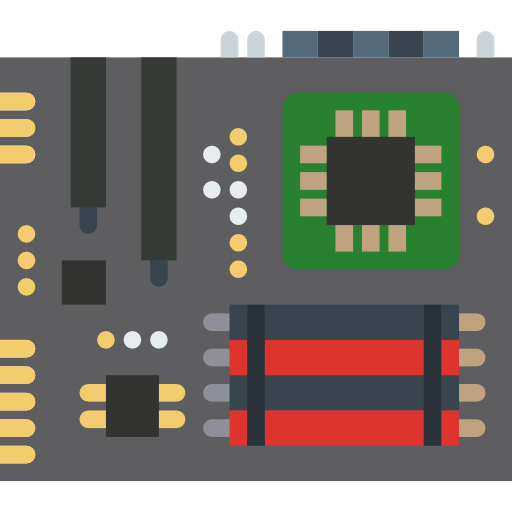
\includegraphics[width=.10\textwidth]{Simulation_sayem/pictures/motherboard.png}};  
\node<2->[inner sep=0pt] (videocard) at (6,0)
    {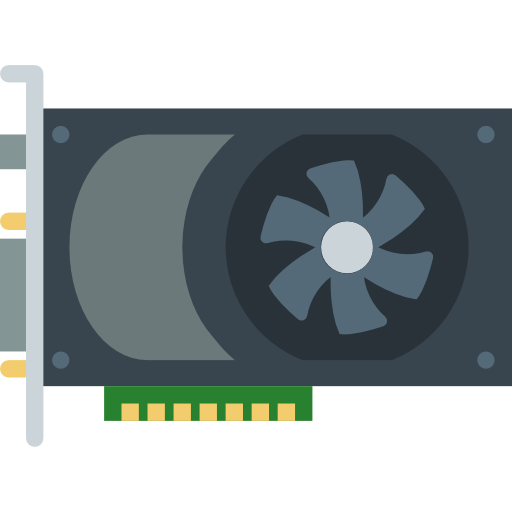
\includegraphics[width=.10\textwidth]{Simulation_sayem/pictures/video-card.png}};
    
\node<2->[inner sep=0pt] (memory) at (2,0)
    {
\includegraphics[width=.10\textwidth]{Simulation_sayem/pictures/memory.png}};
    
\node<2->[inner sep=0pt] (casing) at (10,0)
    {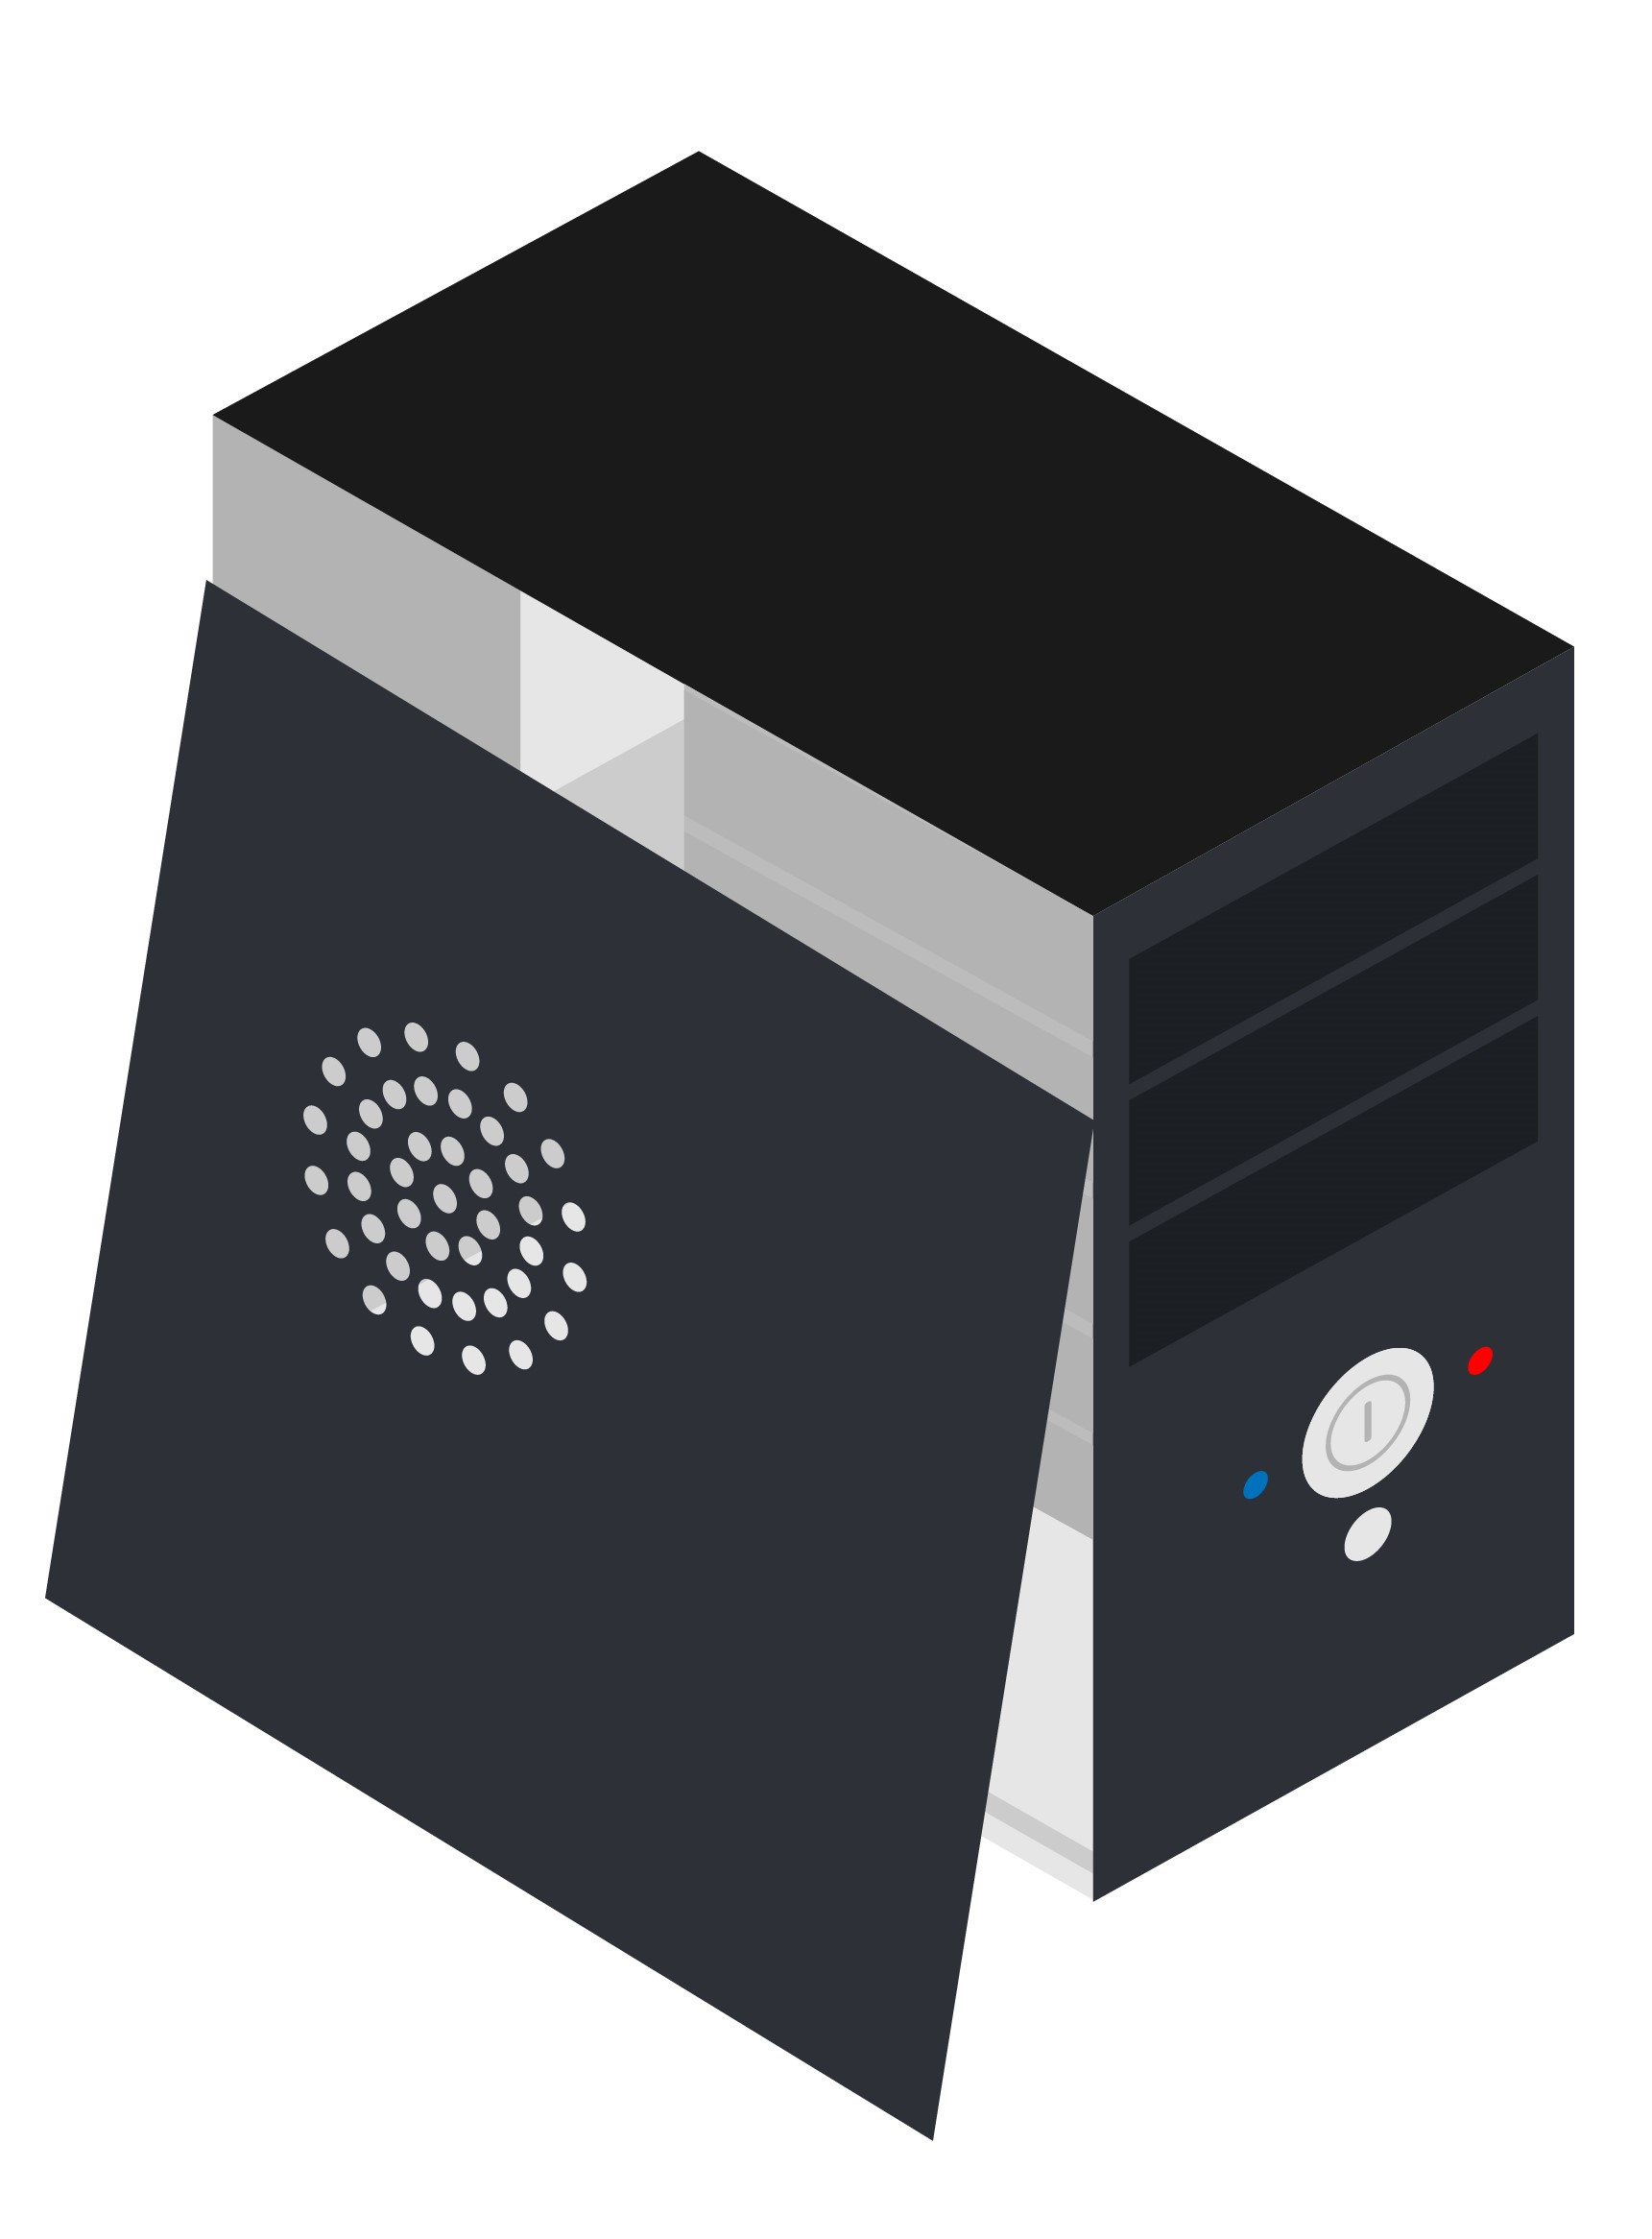
\includegraphics[width=.10\textwidth]{Simulation_sayem/pictures/casing.jpg}};
\node<2->[inner sep=0pt] (PSU) at (8,0)
    {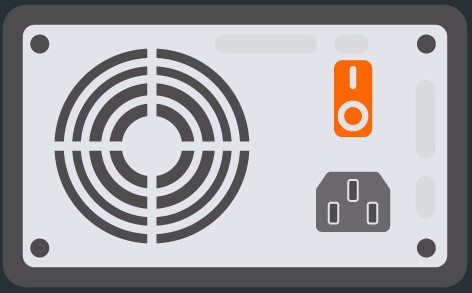
\includegraphics[width=.10\textwidth]{Simulation_sayem/pictures/powerSupply.jpg}};
\node<2->[inner sep=0pt] (CPU) at (4,0)
    {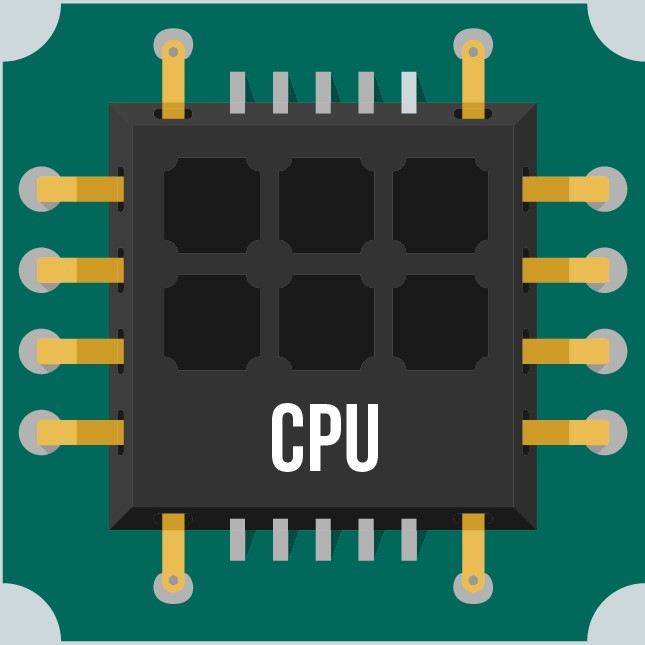
\includegraphics[width=.06\textwidth]{Simulation_sayem/pictures/processor.jpg}};

\end{tikzpicture}

\end{textblock}


\begin{textblock}{14}(2,7)
    \begin{itemize}
        \item[]<2->RAM can be bought right after motherboard
    \end{itemize}
    

\end{textblock}




\begin{textblock}{14}(2,9)
    \begin{itemize}
    \item<3-> Dependencies should be taken care beforehand \\
    In our example, we could not buy casing before motherboard and PSU
\end{itemize}
\end{textblock}
